
\documentclass[10pt,xcolor=table]{beamer}

\usepackage{graphicx}
\usepackage{caption}
\usepackage{subcaption}

% \usepackage[utf8]{inputenc}
% \usepackage[T1]{fontenc}
\usepackage[table]{xcolor}    % loads also »colortbl«
%  \usepackage{enumitem}
\usepackage{ucltemplate}
\usepackage{color}

\usepackage{pgfgantt} % for grantt charts
\usepackage{rotating}
\usepackage[graphicx]{realboxes}

\usepackage{tikz}
\usetikzlibrary{arrows,positioning, shapes.symbols,shapes.callouts,patterns,shapes,chains,calc,backgrounds,fadings}


\setbeamersize{text margin left=15pt,text margin right=15pt,text margin bottom=15pt}


\begin{document}

\frame{\titlepage}

\setbeamerfont{frametitle}{size=\large}

\begin{frame}
\frametitle{Method}

\newcommand{\lw}{0.5mm}
% \newcommand{\mycirc}[2]{\draw (#1,#2) circle (3cm);}

\newcommand{\outFolder}{.}

\begin{columns}[T]
    \hspace{-3em}
    \begin{column}{.5\textwidth}
     %\begin{block}{}
    Model fitting with EM:
    \begin{enumerate}
    \item Estimate vertex assignment to clusters
    \item Refine trajectories
    \item Refine subject stages
    \end{enumerate}
    %\end{block}
    \end{column}
    \hspace{-5em}
    \begin{column}{.5\textwidth}
    %\begin{block}{}


    \begin{figure}
    \centering
    \begin{tikzpicture}
     \draw[line width=\lw] (-0.1,0) arc (-20:20:2) node (A1) {};
     \draw[line width=\lw] (1.7,0) arc (-20:20:2)  node (A2) {} ;
     \draw[,fill=red] (0.22,0.10) circle (0.15cm);
     \draw[,fill=red] (0.32,0.50) circle (0.15cm);
     \draw[,fill=blue] (0.32,0.90) circle (0.15cm);
     \draw[,fill=red] (0.22,1.30) circle (0.15cm);
     \draw[,fill=red] (0.62,0.10) circle (0.15cm);
     \draw[,fill=blue] (0.72,0.50) circle (0.15cm);
     \draw[,fill=blue] (0.72,0.90) circle (0.15cm);
     \draw[,fill=red] (0.62,1.30) circle (0.15cm);
     \draw[,fill=green] (1.02,0.10) circle (0.15cm);
     \draw[,fill=red] (1.12,0.50) circle (0.15cm);
     \draw[,fill=red] (1.12,0.90) circle (0.15cm);
     \draw[,fill=green] (1.02,1.30) circle (0.15cm);
     \draw[,fill=green] (1.42,0.10) circle (0.15cm);
     \draw[,fill=green] (1.52,0.50) circle (0.15cm);
     \draw[,fill=green] (1.52,0.90) circle (0.15cm);
     \draw[,fill=blue] (1.42,1.30) circle (0.15cm);
     \node (sig0) at (1.20,3.00) {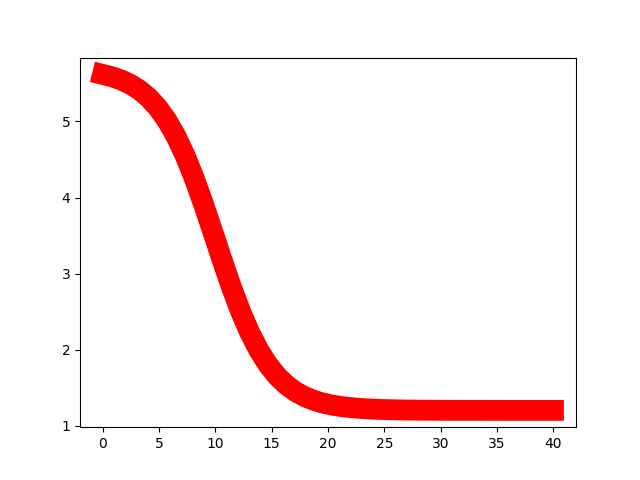
\includegraphics[scale=0.08, trim=70 70 70 0]{\outFolder/sig0.png}};
    \node  (traj) at (sig0.north) {\scriptsize{Traj. 0}}; 
     \node (sig1) at (2.75,2.25) {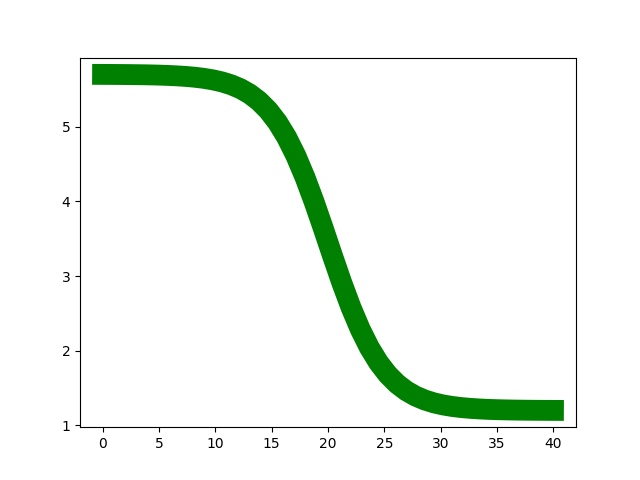
\includegraphics[scale=0.08, trim=70 70 70 0]{\outFolder/sig1.png}};
    \node  (traj) at (sig1.north) {\scriptsize{Traj. 1}}; 
     \node (sig2) at (3.00,0.80) {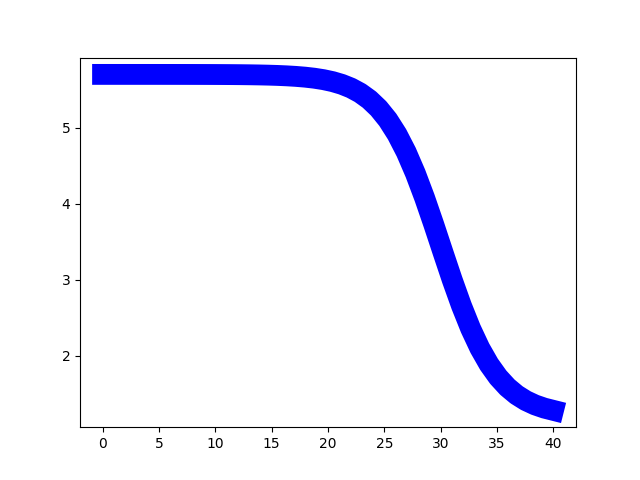
\includegraphics[scale=0.08, trim=70 70 70 0]{\outFolder/sig2.png}};
    \node  (traj) at (sig2.north) {\scriptsize{Traj. 2}}; 


    \draw[dotted, line width=0.6, color=red] (sig0.south west) -- (-0.1,1.5);
    \draw[dotted, line width=0.6, color=red] (sig0.south east) -- (1.8,1.5);

    \draw[dotted, line width=0.6, color=green] (sig1.west) -- (01,1.5);
    \draw[dotted, line width=0.6, color=green] (sig1.south) -- (1.8,0);

    \draw[dotted, line width=0.6, color=blue] (sig2.north west) -- (1.6,1.5);
    \draw[dotted, line width=0.6, color=blue] (sig2.south west) -- (0.7,0.3);

    \node  (vertices_label) at (0.8,1.8) {\scriptsize{Vertices}};


    % draw the bran and the magnification from it
    \node  (brain) at (-2,0.8) {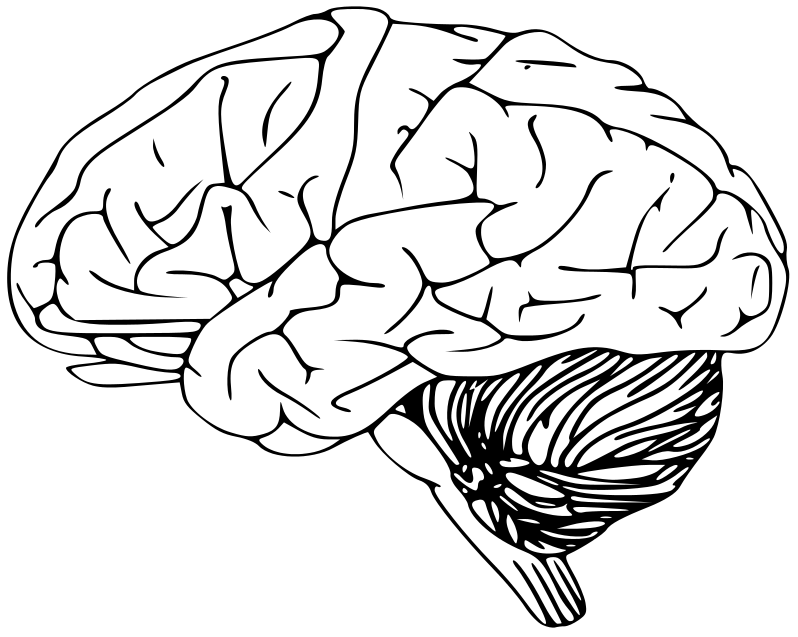
\includegraphics[scale=0.06]{\outFolder/brain.png}};

    \draw (-1.6,1.1) circle (0.15cm) node (C) {};
    \draw[dotted, line width=0.6, color=black] (C.north) -- (A1.west);
    \draw[dotted, line width=0.6, color=black] (C.south) -- (-0.2,0);


   \end{tikzpicture}
  \end{figure}

    %\end{block}
    \end{column}
  \end{columns}

\end{frame}

\end{document}

